\section{Problem definition}
The problem is that traditional rendering methods do not excel at visualizing curved objects, such as quadratic surfaces.
Three-dimensional objects are commonly represented as a triangle mesh, but for quadrics this means that a tesselated approximation has to be generated. 
Any triangle mesh consists of hard-angled edges, thus a mesh representation of a quadric can never be completely smooth.
Finer tesselation will result in a smoother appearance, but at the cost of a higher vertex processing workload.
Despite this, closely zooming in on a triangle mesh will always reveal its angular edges, as Figure \ref{f:glutspheres} illustrates.

Another method for representing spheres is to pre-render them to a 2D depth sprite, which are rendered as a flat billboard in a 3D scene.
This method works for spheres because they look the same from all angles, so using a flat texture that stays faced at the camera is enough to convey the idea that the object is a spherical volume.
The problem with this method is that textures have limited resolution and so depth sprites will become blurry when closely zoomed in.
Also, rendering depth sprites does not take into account deformations of objects caused by perspective projection.

What we need is a method for rendering quadratic surfaces that does not require a coarsely approximated representation of a surface and which produces perspective-correct results, 
while being efficient enough for rendering at real-time speeds.

\begin{figure}[!ht]
\centering
\subfloat[Polygonal tesselation]{\label{f:glutspheres}\resizebox{70mm}{!}{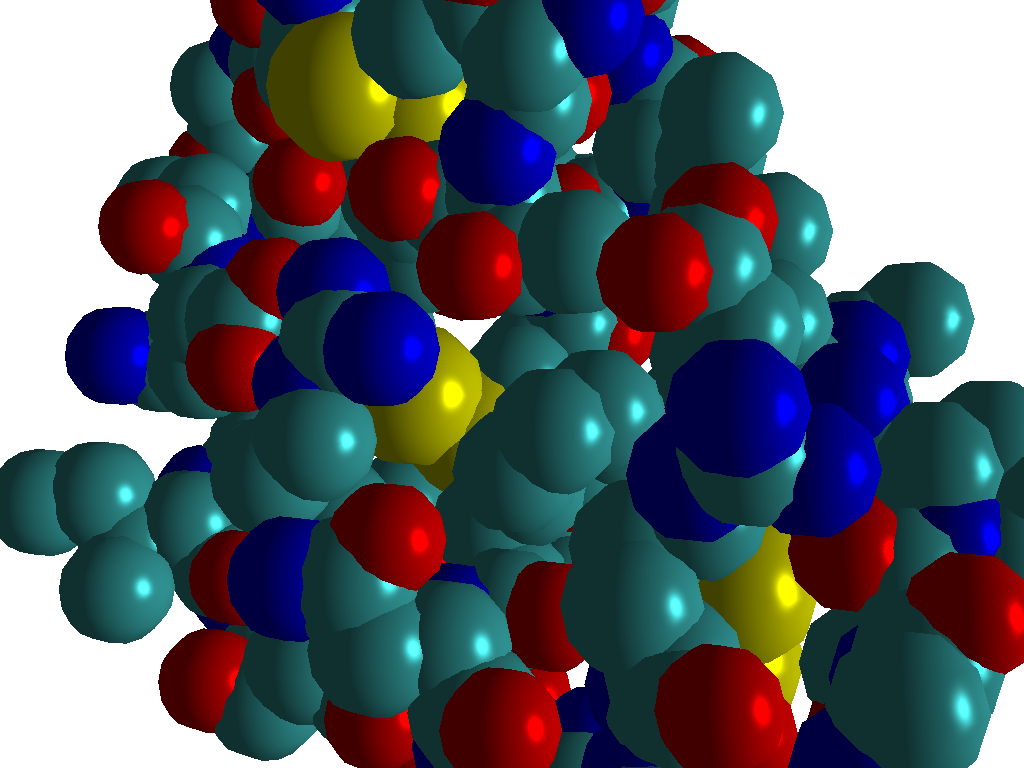
\includegraphics{img/glutspheres.png}}}
\hspace{5mm}\subfloat[Ray-casting]{\resizebox{70mm}{!}{\label{f:rayspheres}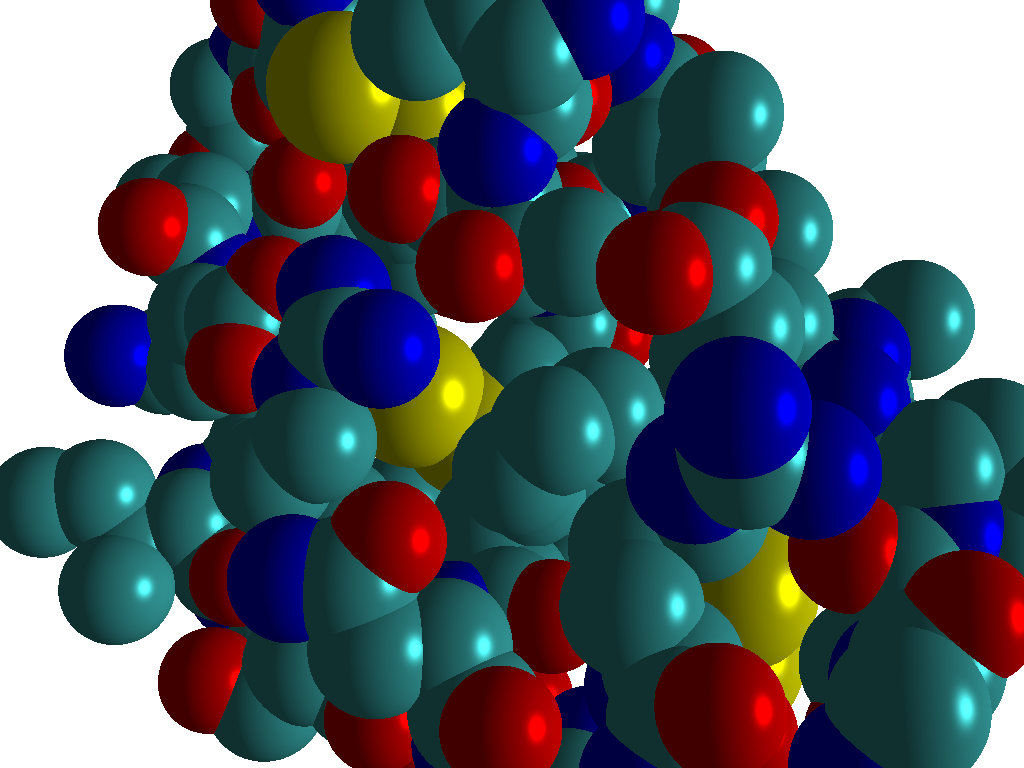
\includegraphics{img/rayspheres.png}}}
\caption{\em Different methods for visualizing spheres. 
Note that the polygonal representation displays angular deformations of the sphere outlines and their specular highlights,
as well as jagged edges where spheres intersect.}
\label{f:methods}
\end{figure}
